\section{Diagnosis Technique}
\label{sec:technique}

\subsection{Overview}

\begin{figure*}[t]
%\todo{In the figure, replace each occurrence of ``clicking'' by ``click''.}
%\todo{Delete ``on Crossword'' in upper left corner.}
%\todo{Use some kind of grouping, such as a horizontal brace, to show that UI
%Action 1 through UI Action 3 are all associated with ``3. Random Action Execution''.}
  \centerline{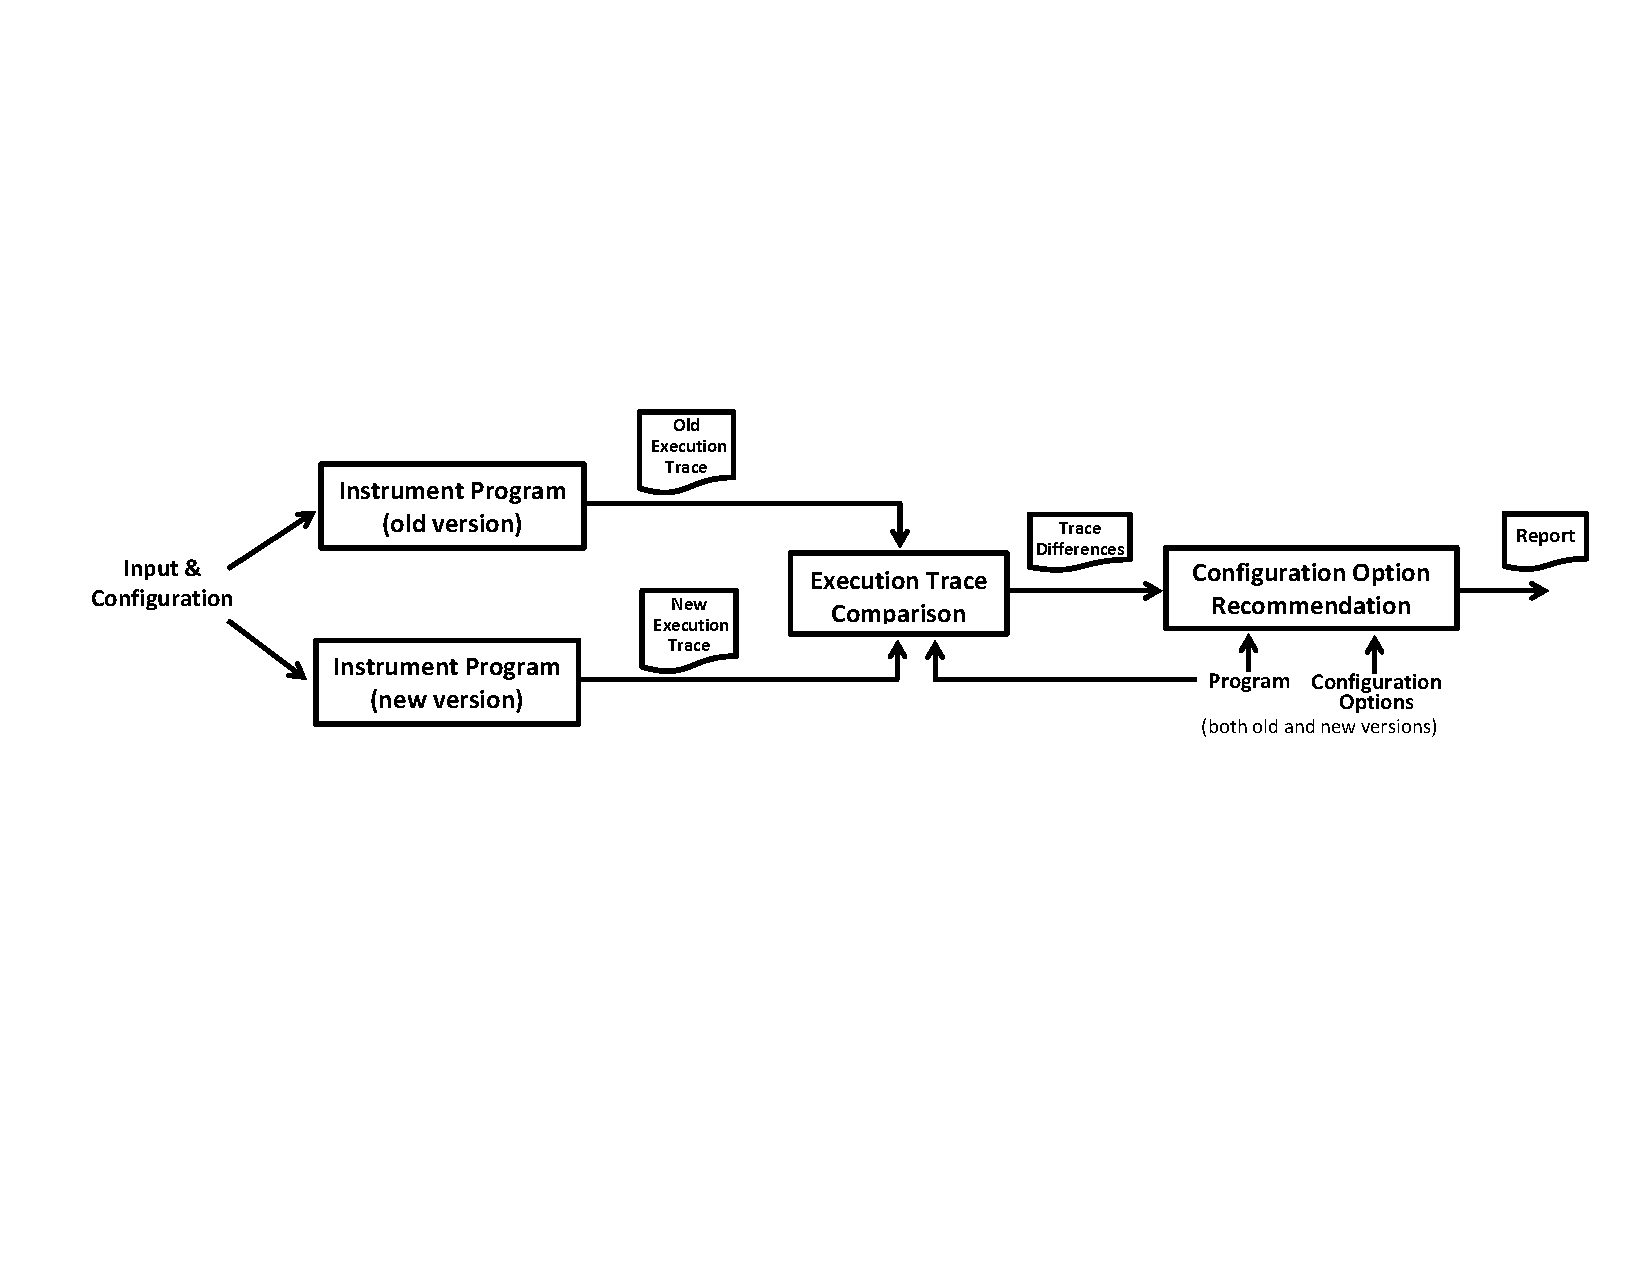
\includegraphics[scale=0.72]{workflow}}
  \vspace*{-2.0ex}\caption {{\label{fig:overview} Workflow..
}}
\end{figure*}


\subsection{Configuration-Aware Instrumentation}

\subsection{Execution Profile Comparison}

The goal is to attribute specific execution differences
to one or more root causes.

\subsubsection{Static Program Matching}

Given a predicate, find the matched predicate in the
new program.

\begin{figure}[t]
\textbf{Axuiliary methods}:

sameStatement($\mathit{s}$, $\mathit{s'}$): return whether two statements
$\mathit{s}$ and $\mathit{s'}$ are the same statements. \todo{What does
  ``same statement'' mean?  The same source code?  The same subexpressions
  too? (For example, does this return true for if statement only if the
  predicate, then clause, and else clause are all identical?)}

BFS($\mathit{s}$, $\mathit{cfg}$): return an ordered list of reachable successive statements from statement $\mathit{s}$ in $\mathit{cfg}$ by Breath-First Search (BFS).

firstMatch($\mathit{stmtList_1}$, $\mathit{stmtList_2}$): return the first matched statement pair between $\mathit{stmtList_1}$ and $\mathit{stmtList_2}$ (iterating $\mathit{stmtList_1}$ first).
\todo{What is a ``matched statement pair''?}


\textbf{Input}: two methods from two software versions: $\mathit{m_{old}}$ and $m_{new}$,

\quad a maximum lookahead value $\mathit{lh}$ (Our experiment uses $\mathit{lh}=5$.).\\
\textbf{Output}: matched statements between old and new versions.
\vspace{-4mm}%
matchStatements($\mathit{m_{old}}$, $\mathit{m_{new}}$, $\mathit{lh}$)\\
\begin{algorithmic}[1]
\STATE $\mathit{matchedStmts}$ $\leftarrow$ new Map$\langle$Stmt, Stmt$\rangle$
\STATE $\mathit{cfg_{old}}$ $\leftarrow$ constructControlFlowGraph($\mathit{m_{old}}$)
\STATE $\mathit{cfg_{new}}$ $\leftarrow$ constructControlFlowGraph($\mathit{m_{new}}$)
\STATE $\mathit{stack}$ $\leftarrow$ new Stack$\langle$Pair$\langle$Stmt, Stmt$\rangle$$\rangle$
\STATE $\mathit{stack}$.push($\mathit{cfg_{old}}$.$\mathit{entry}$, $\mathit{cfg_{new}}$.$\mathit{entry}$)
\WHILE{$\mathit{stack}$ is not empty}
\STATE $\langle$$\mathit{stmt_{old}}$, $\mathit{stmt_{new}}$$\rangle$ $\leftarrow$ $\mathit{stack}$.pop()
%\IF{$\mathit{stmt_{old}}$ or $\mathit{stmt_{new}}$ has already been matched}
\IF{$\mathit{matchedStmts}$.keys().contains($\mathit{stmt_{old}}$) \\ \quad || $\mathit{matchedStmts}$.values().contains($\mathit{stmt_{new}}$)}
\STATE \textbf{continue}
\ENDIF
\IF{sameStatement($\mathit{stmt_{old}}$, $\mathit{stmt_{new}}$)}
\STATE $\mathit{matchedStmts}$[$\mathit{stmt_{old}}$] $\leftarrow$ $\mathit{stmt_{new}}$
\ELSE
\STATE $\mathit{stmtList_{old}}$ $\leftarrow$ BFS($\mathit{stmt_{old}}$, $\mathit{lh}$)
\STATE $\mathit{stmtList_{new}}$ $\leftarrow$ BFS($\mathit{stmt_{new}}$, $\mathit{lh}$)
\STATE $\langle$$\mathit{stmt_{old}}$, $\mathit{stmt_{new}}$$\rangle$ $\leftarrow$ firstMatch($\mathit{stmtList_{old}}$, $\mathit{stmtList_{new}}$)
\IF{$\langle$$\mathit{stmt_{old}}$, $\mathit{stmt_{new}}$$\rangle$ $\neq$ null}
\STATE $\mathit{stack}$.push($\langle$$\mathit{stmt_{old}}$, $\mathit{stmt_{new}}$$\rangle$)
\ENDIF
\ENDIF
\ENDWHILE
\RETURN $\mathit{matchedStmts}$
\end{algorithmic}
\vspace{-4mm}
\caption{Algorithm for matching statements from two methods.
\label{fig:matching}
\todo{This algorithm is suspicious to me.  For one thing, the size of the
  stack is always $\le 1$ --- why use a stack in that case?  For another
  thing, as soon as \emph{any} statement satisfies sameStatement(), then
  the algorithm terminates.  Is there a bug in the algorithm?}
}
\end{figure}


\subsubsection{Dynamic Trace Comparison}

An alternate path is any path not taken by the actual
program execution that starts at a conditional
branch instruction for which the branch condition
is affected by one or more configuration options.

\subsection{Root Cause Analysis}

what about 

if(a) \{

    if(b) \{
        //should a and b equally important
     \}

    \}

\subsubsection{Configuration Option Identification}

Essentially, this step answers the question:
``how likely is it that changing a configuration
option would have prevented this event
from executing?''.
\ourtool uses two heuristics: xxx.
These heuristics cause real root causes to rank
higher than false positives.


\ourtool next determines why each different path
gets executed. \ourtool associates each block
with a set of root causes, More specifically,
it uses thin slicing to identify a
set of configuration options for each deviated
execution path as the root causes.


\ourtool propagates configuration options xx to
other locations in the program according to the
dependencies introduced via data and control flow.
Rather than tracking as a binary value, \ourtool
associates a floating-point weight (between
zero and one) with each configuration option
as its effects propagates in the program.
The weight represents the strength of the causual
relationship between the configuration option
and the execution path.

(using floating-point weight is necessary)

Two configuration options are considered equal
root causes even if one has a direct causal
relationship to a location (e.g., the value
in memory was read directly from the configuration value)
and another has a nebulous relationship (e.g., 
its effects is propagated along a long chain
of conditional assignments).

Data flow dependencies are treated to be more likely
to lead to the root cause than control flow
dependencies. Control flow dependencies are assumed
to be more likely to the root cause if they occur
later in the execution (i.e., closer to the
deviated execution paths).

Assign control flow dependence only half the weight
of the weight introduced by data flow dependencies.
Further, each nested conditional branches reduces
the weight by prior branch in the nest one half.

\subsubsection{Difference Summarization}


\begin{figure}[t]
\textbf{Auxiliary methods:}

\quad getAffectingOptions($\mathit{p}$, $\mathit{V}$): return all configuration options that affect predicate $\mathit{p}$ in the software version $\mathit{V}$

\quad getExecutedStmtNum($\mathit{p}$, $\mathit{V}$, $\mathit{T}$): return the number of executed statements (determined by predicate $\mathit{p}$) in trace $\mathit{T}$

\textbf{Input}: two software version: $\mathit{V_{old}}$ and $\mathit{V_{new}}$, 

\quad the map of all behaviorally-deviated predicates: $\mathit{predMap}$, produced by Figure~\ref{fig:identify}.

\textbf{Output}: {a ranked list of likely root cause configuration options}
\vspace{-4mm}%
recommendOptions($\mathit{V_{old}}$, $\mathit{V_{new}}$, $\mathit{predMap}$)\\
\begin{algorithmic}[1]
\STATE $\mathit{optionMap}$ $\leftarrow$ new Map$\langle$Option, Float$\rangle$
\FOR{each $\langle$$\mathit{p_{old}}$, $\mathit{p_{new}}$$\rangle$ in $\mathit{predMap}$.keys()}
\STATE $\mathit{v}$ $\leftarrow$ $\mathit{predMap}$[$\langle$$\mathit{p_{old}}$, $\mathit{p_{new}}$$\rangle$]
\IF{$\mathit{p_{old}}$ $\neq$ $\mathit{null}$}
\STATE $\mathit{options_{old}}$ $\leftarrow$ getAffectingOptions($\mathit{p_{old}}$, $\mathit{V_{old}}$)
\STATE $\mathit{v}$ $\leftarrow$ $\mathit{v}$ $\times$ getExecutedStmtNum($\mathit{p_{old}}$, $\mathit{V_{old}}$, $\mathit{T_{old}}$)
\FOR{each Option $\mathit{option}$ in $\mathit{options_{old}}$}
\STATE $\mathit{optionMap}$[$\mathit{option}$] = $\mathit{optionMap}$[$\mathit{option}$] + $\mathit{v}$
\ENDFOR
\ENDIF
\IF{$\mathit{p_{new}}$ $\neq$ $\mathit{null}$}
\STATE $\mathit{options_{new}}$ $\leftarrow$ getAffectingOptions($\mathit{p_{new}}$, $\mathit{V_{new}}$)
\STATE $\mathit{v}$ $\leftarrow$ $\mathit{v}$ $\times$ getExecutedStmtNum($\mathit{p_{new}}$, $\mathit{V_{new}}$, $\mathit{T_{new}}$)
\FOR{each Option $\mathit{option}$ in $\mathit{options_{new}}$}
\STATE $\mathit{optionMap}$[$\mathit{option}$] = $\mathit{optionMap}$[$\mathit{option}$] + $\mathit{v}$
\ENDFOR
\ENDIF
\ENDFOR
\RETURN $\mathit{optionMap}$.sortedKeys()
\vspace{-2mm}
\end{algorithmic}
\caption{Algorithm for recommending configuration options.
\label{fig:recommend}
}
\end{figure}


\todo{mention implementation details about recursive, avoid double count}

\ourtool uses the number of instructions in a basic
block as a metric to characterize the execution path.
\todo{xxx}

The block's execution depends on the value of
the configuration option, and the associated weight
indicates the strength of the dependency.


\ourtool also tracks implicit control flow dependencies.

It assumes that control flow dependencies are more likely
to lead to the root cause if they
occur closer to the basic block being executed.

This represents the belief that the execution of
the basic block is affected by XXX.
Since these are two independent probabilities:
potentially changing either of the two options
might cause the basic block to not have been executed.
Thus, the weights of configuration options associated
with a basic block need not sum to one.

\ourtool determines the root cause of each divergence.
It attributes the cost of the divergence (xxx executed
basic block) to the associated configuration options.
It calculates a cost for the divergence by first summing
the costs of all basic blocks along the divergent
path. It attributes the divergence
to root cause configuration options by multiplying
the cost of the divergence by the weights of the configuration
options that are relevant to the divergence.
the 

\todo{repeatedly applying thin slicing is different than full slicing.}


\subsection{Discussion}

This paper

\todo{test case passes, configuration option
may not be thought of}

\ourtool currently assumes that only one
configuration option has an incorrect value.
If fixing a particular configuration error
requires changing values of two configuration options,
then \ourtool may not identify both of them.


Deterministic, not multithreaded

Exclude libraries

\noindent \textbf{Cases that \ourtool may not work well.}
Containing lots of redundant computation that have
little effect to the output, and such redundant computation
is not controlled by any configuration option.
This is highly unlikely for realistic programs.

\noindent \textbf{Why not use dynamic slicing?} The code
omission problem. Some omitted code may lead to
other code omitted.
